\documentclass[border=10pt]{standalone}
\usepackage{tikz}
\usepackage{amsmath,amssymb}
\usetikzlibrary{arrows.meta,positioning,shapes.geometric,fit,calc,decorations.pathmorphing,backgrounds}

% Forgis brand colors — academic palette for white-background figures
% Source: color_schema.json
%
% Usage: % Forgis brand colors — academic palette for white-background figures
% Source: color_schema.json
%
% Usage: % Forgis brand colors — academic palette for white-background figures
% Source: color_schema.json
%
% Usage: \input{colors.tex} in each standalone figure .tex file.
% All figures MUST use only these colors. No inline hex.

% Brand primaries
\definecolor{ctiger}{HTML}{FF5A00}       % Primary accent (Forgis orange)
\definecolor{cfire}{HTML}{FF4D00}        % Critical
\definecolor{cflicker}{HTML}{DC4B07}     % Secondary accent
\definecolor{csteel}{HTML}{878F92}       % Muted neutral
\definecolor{cgunmetal}{HTML}{122128}    % Dark text

% Academic derived palette
\definecolor{cprimary}{HTML}{FF5A00}     % = tiger
\definecolor{cprimarylight}{HTML}{FF8C42}
\definecolor{cprimarybg}{HTML}{FFF0E6}
\definecolor{csecondary}{HTML}{2B6CB0}   % Complementary blue
\definecolor{csecondarylight}{HTML}{4A90D9}
\definecolor{csecondarybg}{HTML}{E8F0FA}
\definecolor{caccent}{HTML}{2D8A6E}      % Teal
\definecolor{caccentlight}{HTML}{5BB89A}
\definecolor{caccentbg}{HTML}{E6F5F0}
\definecolor{chighlight}{HTML}{DC4B07}   % = flicker
\definecolor{chighlightbg}{HTML}{FDEDE6}
\definecolor{ctextdark}{HTML}{122128}    % = gunmetal
\definecolor{ctextmid}{HTML}{878F92}     % = steel
\definecolor{ctextlight}{HTML}{B0B7BA}
\definecolor{cborder}{HTML}{D1D5D8}
\definecolor{cbgwarm}{HTML}{FFF8F2}
\definecolor{cbgcool}{HTML}{F4F7FA}
 in each standalone figure .tex file.
% All figures MUST use only these colors. No inline hex.

% Brand primaries
\definecolor{ctiger}{HTML}{FF5A00}       % Primary accent (Forgis orange)
\definecolor{cfire}{HTML}{FF4D00}        % Critical
\definecolor{cflicker}{HTML}{DC4B07}     % Secondary accent
\definecolor{csteel}{HTML}{878F92}       % Muted neutral
\definecolor{cgunmetal}{HTML}{122128}    % Dark text

% Academic derived palette
\definecolor{cprimary}{HTML}{FF5A00}     % = tiger
\definecolor{cprimarylight}{HTML}{FF8C42}
\definecolor{cprimarybg}{HTML}{FFF0E6}
\definecolor{csecondary}{HTML}{2B6CB0}   % Complementary blue
\definecolor{csecondarylight}{HTML}{4A90D9}
\definecolor{csecondarybg}{HTML}{E8F0FA}
\definecolor{caccent}{HTML}{2D8A6E}      % Teal
\definecolor{caccentlight}{HTML}{5BB89A}
\definecolor{caccentbg}{HTML}{E6F5F0}
\definecolor{chighlight}{HTML}{DC4B07}   % = flicker
\definecolor{chighlightbg}{HTML}{FDEDE6}
\definecolor{ctextdark}{HTML}{122128}    % = gunmetal
\definecolor{ctextmid}{HTML}{878F92}     % = steel
\definecolor{ctextlight}{HTML}{B0B7BA}
\definecolor{cborder}{HTML}{D1D5D8}
\definecolor{cbgwarm}{HTML}{FFF8F2}
\definecolor{cbgcool}{HTML}{F4F7FA}
 in each standalone figure .tex file.
% All figures MUST use only these colors. No inline hex.

% Brand primaries
\definecolor{ctiger}{HTML}{FF5A00}       % Primary accent (Forgis orange)
\definecolor{cfire}{HTML}{FF4D00}        % Critical
\definecolor{cflicker}{HTML}{DC4B07}     % Secondary accent
\definecolor{csteel}{HTML}{878F92}       % Muted neutral
\definecolor{cgunmetal}{HTML}{122128}    % Dark text

% Academic derived palette
\definecolor{cprimary}{HTML}{FF5A00}     % = tiger
\definecolor{cprimarylight}{HTML}{FF8C42}
\definecolor{cprimarybg}{HTML}{FFF0E6}
\definecolor{csecondary}{HTML}{2B6CB0}   % Complementary blue
\definecolor{csecondarylight}{HTML}{4A90D9}
\definecolor{csecondarybg}{HTML}{E8F0FA}
\definecolor{caccent}{HTML}{2D8A6E}      % Teal
\definecolor{caccentlight}{HTML}{5BB89A}
\definecolor{caccentbg}{HTML}{E6F5F0}
\definecolor{chighlight}{HTML}{DC4B07}   % = flicker
\definecolor{chighlightbg}{HTML}{FDEDE6}
\definecolor{ctextdark}{HTML}{122128}    % = gunmetal
\definecolor{ctextmid}{HTML}{878F92}     % = steel
\definecolor{ctextlight}{HTML}{B0B7BA}
\definecolor{cborder}{HTML}{D1D5D8}
\definecolor{cbgwarm}{HTML}{FFF8F2}
\definecolor{cbgcool}{HTML}{F4F7FA}


\begin{document}
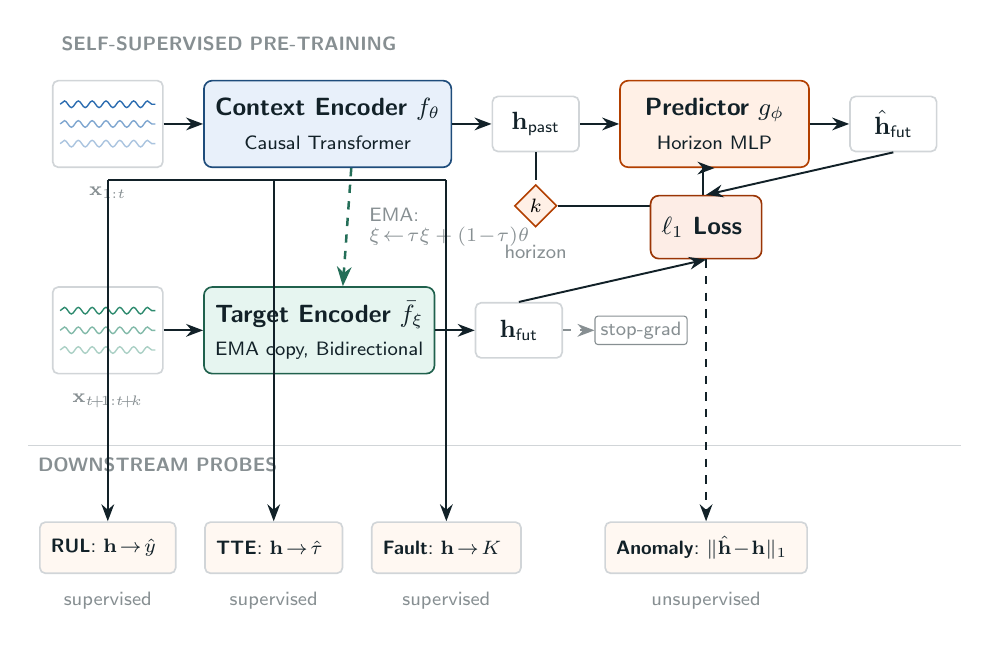
\begin{tikzpicture}[
    >=Stealth,
    font=\sffamily\small,
    % Data-flow arrows: solid, dark
    dataarrow/.style={->,line width=0.7pt,ctextdark},
    % Non-data arrows: dashed, muted
    metaarrow/.style={->,line width=0.7pt,dashed,ctextmid},
    % Main encoder/predictor blocks
    mainblock/.style={
        rounded corners=3pt,
        line width=0.6pt,
        minimum height=1.1cm,
        minimum width=2.4cm,
        align=center,
        text=ctextdark,
        inner sep=4pt,
    },
    % Small representation capsules
    capsule/.style={
        rounded corners=2pt,
        draw=cborder,
        fill=white,
        line width=0.6pt,
        minimum height=0.7cm,
        minimum width=1.1cm,
        align=center,
        text=ctextdark,
        inner sep=4pt,
    },
    % Input signal box
    inputbox/.style={
        rounded corners=2pt,
        draw=cborder,
        fill=white,
        line width=0.6pt,
        minimum height=1.1cm,
        minimum width=1.4cm,
        align=center,
        text=ctextdark,
        inner sep=4pt,
    },
    % Downstream probe boxes
    probe/.style={
        rounded corners=2pt,
        draw=cborder,
        fill=cbgwarm,
        line width=0.6pt,
        minimum height=0.65cm,
        minimum width=1.6cm,
        align=center,
        text=ctextdark,
        inner sep=4pt,
    },
    % Annotation text
    annot/.style={font=\sffamily\scriptsize,text=ctextmid},
    % Section headers
    sechead/.style={font=\sffamily\scriptsize\bfseries,text=ctextmid},
]

% ============================================================
% TOP ROW: Context branch (self-supervised pre-training)
% ============================================================

% --- Input x_{1:t} ---
\node[inputbox] (ctx_input) {};

% Wavy sensor lines inside (blue/context coloring)
\begin{scope}
    \clip ([xshift=2pt,yshift=2pt]ctx_input.south west)
        rectangle ([xshift=-2pt,yshift=-2pt]ctx_input.north east);
    \foreach \yoff/\col in {0.25/csecondary,0.0/csecondary!60,-0.25/csecondary!40} {
        \draw[\col,line width=0.5pt,
              decorate,decoration={snake,amplitude=1.2pt,segment length=5pt}]
            ([xshift=3pt,yshift=\yoff cm]ctx_input.west)
            -- ([xshift=-3pt,yshift=\yoff cm]ctx_input.east);
    }
\end{scope}
\node[annot,below=0.12cm of ctx_input] {$\mathbf{x}_{1:t}$};

% --- Context Encoder f_theta ---
\node[mainblock,
      draw=csecondary!70!black,
      fill=csecondarybg,
      right=0.5cm of ctx_input] (ctx_enc) {
    \textbf{Context Encoder}~$f_\theta$\\[1pt]
    {\scriptsize Causal Transformer}
};
\draw[dataarrow] (ctx_input.east) -- (ctx_enc.west);

% --- h_past capsule ---
\node[capsule,right=0.5cm of ctx_enc] (h_past) {$\mathbf{h}_{\text{past}}$};
\draw[dataarrow] (ctx_enc.east) -- (h_past.west);

% --- Horizon k diamond ---
\node[diamond,
      draw=cprimary!70!black,
      fill=cprimarybg,
      line width=0.6pt,
      inner sep=1.5pt,
      below=0.4cm of h_past,
      anchor=north] (horizon) {{\scriptsize $k$}};
\node[annot,below=0.1cm of horizon] {horizon};

% --- Predictor g_phi ---
\node[mainblock,
      draw=cprimary!70!black,
      fill=cprimarybg,
      right=0.5cm of h_past] (predictor) {
    \textbf{Predictor}~$g_\phi$\\[1pt]
    {\scriptsize Horizon MLP}
};
\draw[dataarrow] (h_past.east) -- (predictor.west);

% Horizon k feeds into predictor bottom
\draw[dataarrow] (horizon.east) -| ([xshift=-0.15cm]predictor.south)
    -- (predictor.south);

% --- Predicted representation ---
\node[capsule,right=0.5cm of predictor] (h_fut_hat) {$\hat{\mathbf{h}}_{\text{fut}}$};
\draw[dataarrow] (predictor.east) -- (h_fut_hat.west);


% ============================================================
% BOTTOM ROW: Target branch
% ============================================================

% --- Input x_{t+1:t+k} ---
\node[inputbox,below=1.5cm of ctx_input] (tgt_input) {};

% Wavy sensor lines (teal/target coloring)
\begin{scope}
    \clip ([xshift=2pt,yshift=2pt]tgt_input.south west)
        rectangle ([xshift=-2pt,yshift=-2pt]tgt_input.north east);
    \foreach \yoff/\col in {0.25/caccent,0.0/caccent!60,-0.25/caccent!40} {
        \draw[\col,line width=0.5pt,
              decorate,decoration={snake,amplitude=1.2pt,segment length=5pt}]
            ([xshift=3pt,yshift=\yoff cm]tgt_input.west)
            -- ([xshift=-3pt,yshift=\yoff cm]tgt_input.east);
    }
\end{scope}
\node[annot,below=0.12cm of tgt_input] {$\mathbf{x}_{t\!+\!1:t\!+\!k}$};

% --- Target Encoder f_bar_xi ---
\node[mainblock,
      draw=caccent!70!black,
      fill=caccentbg,
      right=0.5cm of tgt_input] (tgt_enc) {
    \textbf{Target Encoder}~$\bar{f}_\xi$\\[1pt]
    {\scriptsize EMA copy, Bidirectional}
};
\draw[dataarrow] (tgt_input.east) -- (tgt_enc.west);

% --- h_fut capsule ---
\node[capsule,right=0.5cm of tgt_enc] (h_fut) {$\mathbf{h}_{\text{fut}}$};
\draw[dataarrow] (tgt_enc.east) -- (h_fut.west);

% --- Stop-gradient marker ---
\node[annot,
      draw=ctextmid,
      rounded corners=1pt,
      line width=0.4pt,
      inner sep=2pt,
      right=0.4cm of h_fut] (stopgrad) {stop-grad};
\draw[metaarrow] (h_fut.east) -- (stopgrad.west);


% ============================================================
% EMA arrow: context encoder -> target encoder
% ============================================================

\draw[metaarrow,line width=0.9pt,caccent!80!black]
    ([xshift=0.3cm]ctx_enc.south) -- ([xshift=0.3cm]tgt_enc.north)
    node[midway,right=0.15cm,annot,align=left]
    {EMA:\\[-1pt]$\xi \!\leftarrow\! \tau\xi + (1\!-\!\tau)\theta$};


% ============================================================
% LOSS NODE (between h_fut_hat and h_fut)
% ============================================================

\node[mainblock,
      draw=chighlight!70!black,
      fill=chighlightbg,
      minimum height=0.8cm,
      minimum width=1.4cm,
      inner sep=4pt]
    (loss) at ($(h_fut_hat.south)!0.5!(h_fut.north)$) {
    \textbf{$\ell_1$ Loss}
};
\draw[dataarrow] (h_fut_hat.south) -- (loss.north);
\draw[dataarrow] (h_fut.north) -- (loss.south);


% ============================================================
% SEPARATOR LINE + SECTION LABEL
% ============================================================

\coordinate (sep_y) at ([yshift=-0.9cm]tgt_input.south);

\draw[cborder,line width=0.4pt]
    ([xshift=-0.3cm]ctx_input.west |- sep_y)
    -- ([xshift=0.3cm]h_fut_hat.east |- sep_y);

\node[sechead,anchor=west]
    at ([xshift=-0.3cm,yshift=-0.25cm]ctx_input.west |- sep_y)
    {DOWNSTREAM PROBES};


% ============================================================
% DOWNSTREAM PROBES
% ============================================================

% Probe row y-coordinate
\coordinate (probe_y) at ([yshift=-1.3cm]ctx_input.west |- sep_y);

% --- RUL probe ---
\node[probe] (p_rul) at (ctx_input |- probe_y) {
    {\scriptsize \textbf{RUL}:~$\mathbf{h}\!\to\!\hat{y}$}
};
\node[annot,below=0.1cm of p_rul] {supervised};

% --- TTE probe ---
\node[probe,right=0.35cm of p_rul] (p_tte) {
    {\scriptsize \textbf{TTE}:~$\mathbf{h}\!\to\!\hat{\tau}$}
};
\node[annot,below=0.1cm of p_tte] {supervised};

% --- Fault probe ---
\node[probe,right=0.35cm of p_tte] (p_fault) {
    {\scriptsize \textbf{Fault}:~$\mathbf{h}\!\to\!K$}
};
\node[annot,below=0.1cm of p_fault] {supervised};

% --- Anomaly probe (from loss node) ---
\node[probe] (p_anom) at (loss |- probe_y) {
    {\scriptsize \textbf{Anomaly}:~$\|\hat{\mathbf{h}}\!-\!\mathbf{h}\|_1$}
};
\node[annot,below=0.1cm of p_anom] {unsupervised};

% Fan-out from h_past to RUL, TTE, Fault
% Vertical trunk from h_past
\coordinate (fan_start) at ([yshift=-0.35cm]h_past.south);

\draw[ctextdark,line width=0.7pt] (h_past.south) -- (fan_start);

% Horizontal bus
\coordinate (fan_left) at (fan_start -| p_rul.north);
\coordinate (fan_right) at (fan_start -| p_fault.north);

\draw[ctextdark,line width=0.7pt] (fan_left) -- (fan_right);

% Drop to each probe
\draw[dataarrow] (fan_left) -- (p_rul.north);
\draw[dataarrow] (fan_start -| p_tte.north) -- (p_tte.north);
\draw[dataarrow] (fan_right) -- (p_fault.north);

% Anomaly probe arrow from loss
\draw[dataarrow,dashed] (loss.south)
    -- ([yshift=-0.3cm]loss.south)
    -- ([yshift=-0.3cm]loss.south -| p_anom.north)
    -- (p_anom.north);


% ============================================================
% TOP LABEL
% ============================================================

\node[sechead,anchor=south west]
    at ([yshift=0.25cm]ctx_input.north west)
    {SELF-SUPERVISED PRE-TRAINING};

\end{tikzpicture}
\end{document}
